\section{Physikalische Grundlagen}
Die Ausführungen in diesem Abschnitt orientieren sich an \cite{manual}.

\subsection{Semiklassische Erklärung des Hanle-Effekts}

Semiklassisch wird der Hanle-Effekt folgendermaßen erklärt:
Wenn linear polarisiertes Licht (konstante Richtung von $\vec{\text{E}}$- und $\vec{\text{B}}$-Feld)
ein Atom anregt, ist für dieses angeregte Atom die Richtung seines Dipolmoments $\vec{P}$ vorgegeben:
Es zeigt in Richtung des $\vec{\text{E}}$-Feldes. Senkrecht dazu steht das magnetische Moment $\vec{\mu}$.
\autoref{img:rotation} zeigt den Zusammenhang.\\

\begin{figure}[H]
\begin{center}
  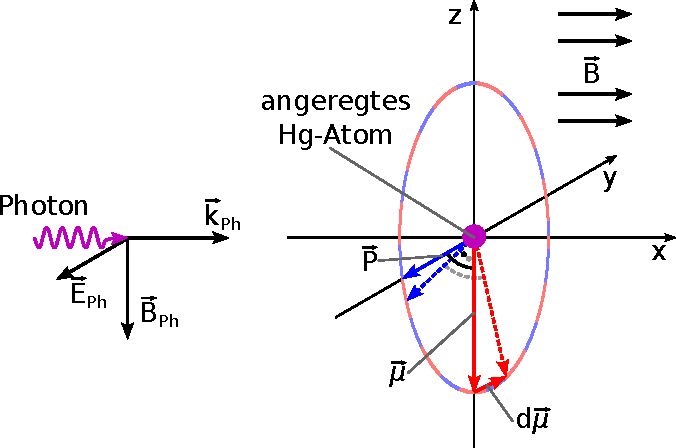
\includegraphics[width=0.5\textwidth]{../img/rotation.pdf}
  \caption{Hanle-Effekt: Präzession des magnetische Moments $\vec{\mu}$ eines angeregten Atoms im
  Magnetfeld $\vec{B}$. Das Dipolmoment $\vec{P}$ steht senkrecht auf $\vec{\mu}$ und rotiert mit.}
  \label{img:rotation}
\end{center}
\end{figure}

Wenn kein äußeres Magnetfeld vorhanden ist,
hat das angeregte Atom die gewöhnliche Abstrahlcharakteristik eines Hertzschen Dipols:
Die Intensität der abgestrahlten Leistung $I$ zeigt eine sin$^2$-Abhängigkeit vom Winkel $\varphi$ zur
Dipolachse:
\begin{equation}
\label{eq:hertz}
I(\varphi) \propto \sin^2(\varphi)
\end{equation} 
\autoref{img:dipol} zeigt diese Abstrahlcharakteristik.

\begin{figure}[H]
\begin{center}
  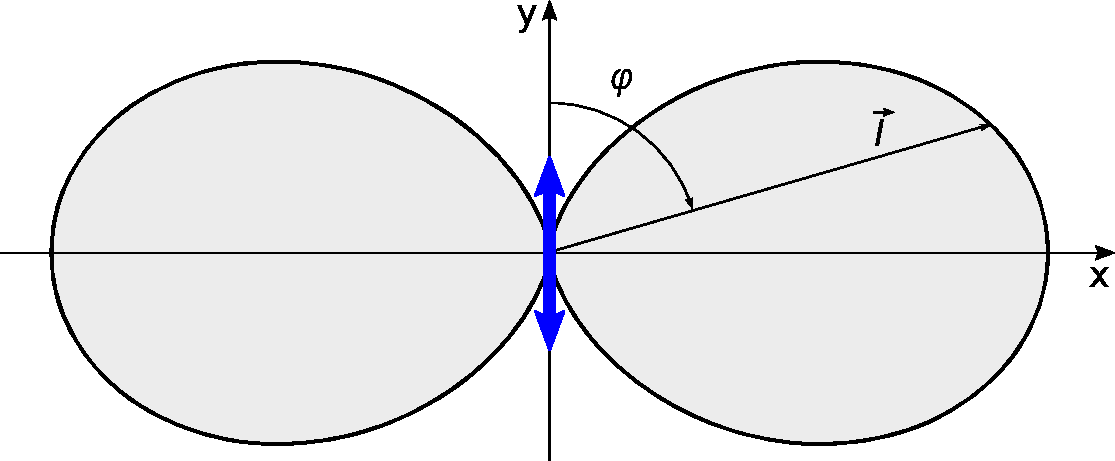
\includegraphics[width=0.6\textwidth]{../img/dipol.pdf}
  \caption{Abstrahlcharakteristik eines Hertzschen Dipols: Strahlungsintensität $\vec{I}$ in Abhängigkeit des
  Winkels $\varphi$.}
  \label{img:dipol}
\end{center}
\end{figure}

Ein einzelnes angeregtes Atom fällt mit der Wahrscheinlichkeit $\exp(-\frac{\tau}{t})$ zurück in den Grundzustand.
(Die mittlere Lebensdauer des angeregten Atoms wird mit $\tau$ bezeichnet, die Anregung findet bei $t = 0$ statt.)
Damit erhält man für die winkelabhängige Gesamtintensität
\begin{equation}
\label{eq:int}
I(\varphi) = A \cdot \int_0^{\infty} \sin^2(\varphi) \cdot \text{e}^{-\frac{\tau}{t}} \ \text{d}t \, \ .
\end{equation}
$A$ ist hier eine Konstante. Befindet sich das angeregte Atom allerdings in einem Magnetfeld $\vec{\text{B}}$,
ist das Integral nicht mehr einfach zu lösen, weil der Winkel $\varphi$ dann zeitabhängig ist.
Dies wird verursacht durch das Drehmoment, das von dem Magnetfeld auf das System ausgeübt wird.
Es gilt
\begin{equation}
\label{eq:dmu}
\frac{\text{d}\vec{\mu}}{\text{d}t} = \frac{\omega_L}{B} \cdot (\vec{\mu} \times \vec{\text{B}}) \ \, .
\end{equation}
Die Änderung von $\vec{\mu}$  führt zu einer Präzession in der Ebene senkrecht zum Magnetfeld
mit der Larmorfrequenz $\omega_L$.
Sie ist abhängig von der Stärke des Magnetfelds, es gilt
\begin{equation}
\label{eq:larmorfreq}
\omega_L = B \cdot \frac{g_J \cdot \mu_B}{\hbar} \ \, .
\end{equation}
Da das Dipolmoment $\vec{P}$ fest mit $\vec{\mu}$ verbunden ist, präzediert auch dieses, und es gilt für den
Winkel
\begin{equation}
\label{eq:phit}
\varphi(t) = \omega_L \cdot t \ \, .
\end{equation}
Die Winkel- und Magnetfeldabhängigkeit der Intensität wird also von folgendem Integral beschrieben:
\begin{equation}
\label{}
I(\Phi,B) = A \cdot \int_0^{\infty} \sin^2 \left( \frac{g_J \cdot \mu_B}{\hbar} \cdot (B-B_0) \cdot t + \Phi \right) \cdot
\text{e}^{-\frac{\tau}{t}} \ \text{d}t + c \, \ .
\end{equation}
$(\Phi + 90^{\circ})$ ist der Winkel zwischen der Polarisationsachse des eingestrahlten Lichts und der Richtung,
in der sich der Strahlungsdetektor befindet.
$A$, $B_0$ und $c$ sind Konstanten, die die Amplitude und Offsets der Messdaten beschreiben.
Die Lösung des Integrals lautet
\begin{equation}
\label{eq:intensity}
I(\Phi,B) = A \tau \cdot \frac{2 a \tau  (B-B_0) \sin (2 \Phi )+(2 a \tau  (B-B_0))^2-\cos (2 \Phi )+1}
{2 \left((2 a \tau  (B-B_0))^2+1\right)}+c \ ,
\end{equation}
mit
\begin{equation}
\label{}
a=\frac{g_J \cdot \mu_B}{\hbar} \, \ .
\end{equation}
Die Lösung ist für $\Phi=0^{\circ}$ eine Lorentzkurve und für $\Phi=90^{\circ}$ eine inverse Lorentzkurve.
\autoref{eq:intensity} wird für die Fits an die Messdaten verwendet.

\subsection{Quantenmechanische Erklärung des Hanle-Effekts}
Der Hanle-Effekt lässt sich auch quantenmechanisch erklären; er ist ein Sonderfall des \emph{level-crossing}. 
Es können mehrere Atomzustände mit derselben Energie existieren, die durch die Feinstrukturaufspaltungen einzelner Zustände (was zu einer Überkreuzung 
dieser führt, \emph{level-crossing}) oder durch das Anlegen eines äußeren Magnetfeldes $B$ (der Hanle-Effekt tritt bei $B=0$), was zur Zeeman-Aufspaltung 
führt, verursacht werden.
Es zeigt sich der Effekt der \emph{Resonanzfluoreszenz}, welcher aus der Interferenz dieser sich überlagernder Zustände folgt. \\
Auf die genaue quantenmechanische Betrachtung soll hier eingegangen werden, es wird auf \cite{manual} verwiesen.



\subsection{\emph{Coherence Narrowing} und Dampfdruck}

Bei der Bestimmung der mittleren Lebensdauer $\tau$ des angeregten Zustands tritt ein Effekt auf,
der das Ergebnis systematisch verfälscht:
Ein Photon, das emittiert wird, wenn ein Atom in den Grundzustand zurückfällt,
kann von einem weiteren Atom absorbiert werden.
Dies führt dazu, dass angeregte Zustände in der Resonanzzelle länger bestehen bleiben,
als ihre Lebensdauer es vorhersagt.
Durch eine Messreihe bei verschiedenen Temperaturen kann die Stärke dieses Effekts bestimmt werden und
man erhält ein bereinigtes Ergebnis.
Man geht davon aus, dass der Effekt proportional zur Anzahl der Quecksilberatome in der Resonanzzelle ist,
also auch proportional zur Partialdruck des Quecksilbers.
Über die Dampfdruckkurve kann der Partialdruck aus der Temperatur der Zelle berechnet werden.
Die Formel dafür lautet
\begin{equation}
\label{eq:vaporpress}
\ln(p/p_{\text{c}})= (T/T_{\text{c}}) \cdot (a_1T_{\text{r}}^{}+a_2T_{\text{r}}^{1.89}+a_3T_{\text{r}}^{2}
+a_4T_{\text{r}}^{8}+a_5T_{\text{r}}^{8.5}+a_6T_{\text{r}}^{9})
\end{equation}
mit $T_{\text{r}}=1-(T/T_{\text{c}})$ und den Parametern



\begin{equation}
\label{eq:params}
\begin{split}
T_{\text{c}} &= 1764\,\text{K} \ \: \qquad a_1=-4.57618  \ \: \qquad a_2=-1.40726        \qquad a_3=2.36264\\
p_{\text{c}} &= 167\,\text{MPa}     \qquad a_4=-31.08800      \qquad a_5=58.01840  \  \qquad a_6=-27.63045
\end{split}
\end{equation}

Die Kovarianzmatrix $C$ für die Parameter lautet (aus \cite{manual})

\begin{equation}
\label{eq:cov}
C=
\left(
\begin{array}{cccccc}
 0.00222 & -0.03976 & 0.03860 & -0.05715 & 0.10490 & -0.04884 \\
 -0.03976 & 0.71363 & -0.69302 & 1.05062 & -1.93198 & 0.90105 \\
 0.03860 & -0.69302 & 0.67305 & -1.0233 & 1.88215 & -0.87799 \\
 -0.05715 & 1.05062 & -1.0233 & 1.80598 & -3.35831 & 1.58313 \\
 0.10490 & -1.93198 & 1.88215 & -3.35831 & 6.24979 & -2.94835 \\
 -0.04884 & 0.90105 & -0.87799 & 1.58313 & -2.94835 & 1.39186 \\
\end{array}
\right)
\end{equation}